% interactcadsample.tex
% v1.03 - April 2017

\documentclass[]{interact}

\usepackage{epstopdf}% To incorporate .eps illustrations using PDFLaTeX, etc.
\usepackage{subfigure}% Support for small, `sub' figures and tables
%\usepackage[nolists,tablesfirst]{endfloat}% To `separate' figures and tables from text if required

\usepackage{natbib}% Citation support using natbib.sty
\bibpunct[, ]{(}{)}{;}{a}{}{,}% Citation support using natbib.sty
\renewcommand\bibfont{\fontsize{10}{12}\selectfont}% Bibliography support using natbib.sty

\theoremstyle{plain}% Theorem-like structures provided by amsthm.sty
\newtheorem{theorem}{Theorem}[section]
\newtheorem{lemma}[theorem]{Lemma}
\newtheorem{corollary}[theorem]{Corollary}
\newtheorem{proposition}[theorem]{Proposition}

\theoremstyle{definition}
\newtheorem{definition}[theorem]{Definition}
\newtheorem{example}[theorem]{Example}

\theoremstyle{remark}
\newtheorem{remark}{Remark}
\newtheorem{notation}{Notation}

% see https://stackoverflow.com/a/47122900

% Pandoc citation processing

\usepackage[hidelinks]{hyperref}
\usepackage[utf8]{inputenc}
\def\tightlist{}
\usepackage{booktabs}
\usepackage{adjustbox}


\begin{document}

\articletype{RESEARCH REPORT - Word count: 2392}

\title{Bayesian Evidence Synthesis}


\author{\name{Thom Benjamin Volker$^{1, 2}$}
\affil{$^{1}$Supervised by Prof.~Dr.~Irene Klugkist; $^{2}$Utrecht
University}
}

\thanks{CONTACT Thom Benjamin
Volker. Email: \href{mailto:t.b.volker@uu.nl}{\nolinkurl{t.b.volker@uu.nl}}}

\maketitle


\begin{keywords}
Bayes factors, Evidence Aggregation, hypothesis evaluation
\end{keywords}

\hypertarget{introduction}{%
\section{Introduction}\label{introduction}}

In recent years, a meta-analytic way of thinking has been advocated in
the scientific community. This approach is grounded in the belief that a
single study is merely contributing to a larger body of evidence
\citep[e.g.,][]{asendorpf_recommendations_2016, cumming_new_2014, goodman_reproducibility_2016, schmidt_replication_2009}.
In this context, the importance of replication has been legitimately
supported
\citep[e.g.,][]{baker_reproducibility_2016, brandt_et_al_replication_2014, munafo_manifesto_2017}.
However, most of the attention has been focused on studies that are
highly similar, using an identical methodology and research design
\citep[e.g.,][]{camerer2016evaluating, camerer2018evaluating, klein_etal_replicability_2014, nosek_replicability_review_2021, open_science_collab_2015}.
These studies, commonly referred to as exact, direct or close
replications, are merely concerned with the statistical reliability of
the results. If the results of the studies depend on methodological
flaws, inferences from all studies will lead to suboptimal or invalid
conclusions \citep{lawlor_triangulation_2017, munafo_robust_2018}.

Conceptual replications, which primarily assess the validity of a study,
protect against placing too much confidence in such flawed findings.
Specifically, conceptual replications are a way of investigating whether
the conclusions hold under alternative conditions, using varying
measurement instruments or other operationalizations
\citep{nosek_scientific_2012}. Different methodologies may have
different strengths and weaknesses, that may affect the final conclusion
that can be drawn from the data. Combining evidence from multiple
approaches mitigates the effect of these strengths and weaknesses, which
enhances the validity and the robustness of the final conclusion
\citep{lawlor_triangulation_2017, lipton2003inference, mathison1988triangulate, munafo_robust_2018, nosek_scientific_2012}.

In the conventional framework of direct replications, combining evidence
over studies is straightforward, because established methods as
(Bayesian) meta-analysis or Bayesian sequential updating can be applied
to aggregate the results
\citep{lipsey_wilson_2001, schonbrodt_sequential_2017, sutton_bayesian_meta2001}.
These methods pool the parameter estimates or effect sizes obtained in
the individual studies \citep{cooper_handbook_2009}. However, if the
studies differ considerably with regard to operationalizations of key
variables or statistical models used, the parameter estimates or effect
sizes will not be comparable. Accordingly, an aggregate of these
estimates cannot be meaningfully interpreted, rendering the use of
conventional methods unfeasible.

To overcome these difficulties, \citet{kuiper_combining_2013} proposed a
new method called \emph{Bayesian Evidence Synthesis} (\emph{BES}). At
its core, \emph{BES} quantifies the support for an overall scientific
theory or an overarching hypothesis, by aggregating Bayes factors
obtained at the level of individual studies. In every single study, a
hypothesis can be formulated that reflects an overall theory, but that
incorporates data characteristics and methodologies unique to that
study. The support for each of these study-specific hypotheses can be
expressed using a Bayes factor (BF), rendering the relative support for
the hypothesis of interest over an alternative hypothesis
\citep{kass_raftery_bayes_factors_1995}. If the study-specific
hypotheses represent the same underlying (i.e., latent) effect, the
Bayes factors in favor of these hypotheses can be meaningfully combined.

Although \emph{BES} has been applied successfully to substantive
research questions
\citep[e.g.,][]{kevenaar_bes_2021, zondervan_parental_2019, zondervan_robust_2020},
hardly any empirical investigation into the method's performance has
been conducted. As a consequence, researchers may be hesitant to
implement the method in practice, because the required conditions to
achieve good performance are relatively unknown. In this paper, it will
be assessed how \emph{BES} behaves empirically when combining evidence
from studies that employ different statistical models, by focusing on
whether \emph{BES} indeed favors true hypotheses over alternatives.
Given the fact that studies with low statistical power (i.e., \(60\%)\)
are omnipresent in social science research
\citep[e.g.,][]{ingre_power_2018, button2013power}, it will be assessed
to what extent \emph{BES} is vulnerable to power issues. Hence, this
paper aims to assess how well \emph{BES} performs when aggregating
results of different analysis techniques, under varying sample sizes and
effect sizes.

\hypertarget{methods}{%
\section{Methods}\label{methods}}

\hypertarget{informative-hypotheses}{%
\subsection{Informative hypotheses}\label{informative-hypotheses}}

At it's core, \emph{BES} aims to quantify the evidence for a scientific
theory, by aggregating the relative amount of evidence for the
hypothesis of interest over multiple studies. A scientific theory is
often best described by an informative hypothesis, which, contrary to
the classical null hypothesis testing approach, allows to make
scientific expectations explicit \citep[e.g.,
see][]{hoijtink_informative_2012, vandeschoot_informative_2011}.\footnote{Other
  advantages of evaluating informative hypotheses are numerous
  \citep[e.g.,
  see][]{beland2012informative, hoijtink_klugkist_boelen_2008, klaassen_informative_2020, vandeschoot_informative_sem_2011, vandeschoot_informative_introduction_2011}.}
As an example, consider a research group investigating whether
researchers who experience more publication pressure are more often
involved in scientific misconduct
\citep[e.g.,][]{gopalakrishna_riet_vink_stoop_wicherts_bouter_2021}.
When putting this theory to the test, the research group may measure the
amount of publication pressure researchers experience and ask how often
these researchers were involved in scientific misconduct, and quantify
both measures on a continuous scale. Formalizing the theory as a
testable informative hypothesis would yield \[
\mathcal{H}_{1}: \beta_{p} > 0,
\] where the hypothesis of interest \(\mathcal{H}_1\) states that the
effect of publication pressure on scientific misconduct \(\beta_{p}\) is
positive. Another researcher might have data in which the outcome,
involvement in scientific misconduct, only consists of two categories
(i.e., ``yes'' or ``no''), but that contains two measures for
publication pressure that are both expected to be positively related to
scientific misconduct: the expected necessity of top-tier publications
for successful grant applications and the expected necessity of top-tier
publications for getting tenure. An expectation might then be that both
sources of publication pressure are positively related to scientific
misconduct, and that the effect of both is actually similar, because
they are equally important to researchers. Capturing this expectation in
an informative hypothesis would yield \[
\mathcal{H}_{2}: \{\beta_{p_1} = \beta_{p_2}\} > 0,
\] where \(\beta_{p_1}\) and \(\beta_{p_2}\) indicate the effect of
publication pressure through grant applications and getting tenure on
scientific misconduct, respectively.

\hypertarget{bayes-factors}{%
\subsection{Bayes factors}\label{bayes-factors}}

The Bayes Factor \citep{kass_raftery_bayes_factors_1995} can be used to
quantify the support for informative hypotheses
\citep{beland2012informative, hoijtink_informative_2012, hoijtink2019tutorial}.
Loosely speaking, a Bayes factor expresses the relative support from the
data for an hypothesis of interest versus some alternative hypothesis.
Returning to the example, the Bayes factor for hypothesis
\(\mathcal{H}_1\) versus an alternative hypothesis \(\mathcal{H}_a\) is
defined as the ratio of the marginal likelihoods of the data under these
hypotheses \[
BF_{1,a} = \frac{P(D|\mathcal{H}_1)}{P(D|\mathcal{H}_a)}.
\] A Bayes factor that equals \(7\) indicates that after seeing the
data, \(\mathcal{H}_1\) is \(7\) times more likely than
\(\mathcal{H}_a\). When the alternative hypothesis is unconstrained
(i.e., \(\mathcal{H}_a = \mathcal{H}_u\)), the expression of the Bayes
factor boils down to \[
BF_{1,u} = \frac{f_1}{c_1},
\] where \(f_1\) indicates the fit of the data to \(\mathcal{H}_1\) and
\(c_1\) indicates the complexity of the hypothesis \(\mathcal{H}_1\)
\citep[e.g.,][]{beland2012informative, klugkist_inequality_2005}. A
similar approach can be used when the hypothesis of interest contains
equality constraints (like hypothesis \(\mathcal{H}_2\) in the example),
but requires some additional steps that will not be discussed here
\citep[see e.g.,][]{mulder_equality_2010, klugkist_inequality_2005}.
When the alternative hypothesis of interest is another informative
hypothesis \(\mathcal{H}_{3}\) (e.g., \(\beta_p < 0\)), the same
formulation of the Bayes factor can be applied to both hypotheses, which
is generally easier than calculating the marginal likelihoods under both
hypotheses \citep{klugkist_inequality_2005}, providing \[
BF_{1,3} = \frac{BF_{1,u}}{BF_{3,u}}.
\] Combining the obtained Bayes factors with prior model probabilities
(i.e., the probability that the hypotheses under consideration are true
\emph{a priori}), allows to calculate posterior model probabilities. The
posterior model probabilities for hypothesis \(\mathcal{H}_i\), with
\(i \in \{1, 2, \dots, m\}\), are given by \[
PMP(\mathcal{H}_{i}) = \frac{\pi_i BF_{i,u}}{\sum^m_{i'=1} \pi_{i'} BF_{i',u}},
\] where \(\pi_i\) indicates the prior model probability of hypothesis
\(H_i\). The posterior model probabilities indicate the relative support
for the hypotheses under consideration.

\hypertarget{bayesian-evidence-synthesis}{%
\subsection{Bayesian evidence
synthesis}\label{bayesian-evidence-synthesis}}

Regardless of differences in study design and analysis plan, a Bayes
factor can be calculated to express the support for the theory in each
of the studies under consideration, as long as the hypotheses under
consideration are conceptually similar. To aggregate the evidence for a
theory over multiple studies, \emph{BES} uses the possibility to specify
the prior model probabilities. After every study that is conducted, the
support for the hypothesis of interest can be expressed as a posterior
model probability. These posterior model probabilities after study \(j\)
can be used as prior model probabilities in study \(j + 1\)
\citep{kuiper_combining_2013}. Independent of the order of updating,
repeating this process for \(J\) studies yields \[
PMP(\mathcal{H}_i)^J = \frac{\pi^0_{i} \prod^J_{j=1} BF^j_{i,u}}{\sum^m_{i'=1} \pi^0_{i'} \prod^J_{j=1} BF^j_{i',u}},
\] where \(\pi^0_i\) indicate the prior model probabilities for
hypothesis \(\mathcal{H}_i\) before a study has been conducted. Because
one could argue that before observing any data all hypotheses are
equally likely, \(\pi^0_i\) is usually the same for all hypotheses
(i.e., \(\pi^0_i = \frac{1}{m}\)). If the initial prior model
probabilities are the same for all hypotheses, the product of Bayes
factors equals the aggregated posterior model odds (the numerator of
\(PMP(\mathcal{H}_i)^J\)), which contains the same information as the
aggregated posterior model probabilities. These measures then indicate
the relative support for the theory (i.e., overall hypothesis) in all
studies simultaneously, irrespective of the specifics of each study.

\hypertarget{simulation}{%
\subsection{Simulation}\label{simulation}}

A simulation study is conducted in \texttt{R} \citep[Version 4.1.0]{R}
to assess how the outcome of \emph{BES} is affected by sample size and
effect size. Because \emph{BES} can be applied regardless of
between-study heterogeneity, data to represent three different studies
is generated using three models: ordinary least squares (OLS), logistic
and probit regression. In all studies, the \emph{true} hypothesis
\(\mathcal{H}_1: \beta_1 < \beta_2 < \beta_3 < \beta_4\) is evaluated
against an unconstrained alternative
\(\mathcal{H}_u: \beta_1, \beta_2, \beta_3, \beta_4\) using the
\texttt{R}-package \texttt{BFpack} \citep[Version 0.3.2]{BFpack}, and
\emph{BES} is used to pool the evidence over studies. Because the
initial prior model probabilities are specified equally (i.e.,
\(\pi^0_1 = \pi^0_u = \frac{1}{2}\)), and the product of Bayes factors
is log-transformed for interpretability, a product that is greater than
\(0\) yields more support for \(\mathcal{H}_1\) than for
\(\mathcal{H}_u\).

Each study consists of a continuous or binary outcome \(Y\) and a
predictor matrix \(X\), with dimensions \(n \times 4\). The sample sizes
vary with \(n \in \{25, 50, 100, 200, 400, 800\}\), while the effect
sizes take on the values \(R^2 \in \{0.02, 0.09, 0.25\}\), in accordance
with small, medium and large effects as defined by \citet{cohen_1988}.
For binary outcomes, McKelvey and Zavoina's \(R^2_{M\&Z}\) is used
\citep{mckelvey_zavoina_1975}, which closely resembles the conventional
\(R^2\) empirically
\citep{hagle_mitchell_goodness_1992, demaris_explained_2002}. Two sets
of simulations will be considered: in the first, the sample sizes and
effect sizes are consistent across studies, while in the second, the
sample size of a single, randomly selected, study is kept fixed at
\(n = 25\). All simulation conditions are evaluated over \(1000\)
iterations. All predictor variables are normally distributed with a mean
of \(0\), a variance of \(1\) and a common covariance of \(0.3\), and
their relation with the outcome \(Y\) is specified according to the
weights-matrix \(B = [1,2,3,4]^T\), such that
\(\beta_4 = 4\beta_1, \beta_3 = 3\beta_1, \beta_2 = 2\beta_1\).
Accordingly the exact coefficients can be defined as \[
\beta = B \Bigg(\sqrt{\frac{\text{Var}(\hat{Y})}{G^T ((B B^T) \odot \Sigma) G }}\Bigg),
\] where \(G\) is a \(4 \times 1\) column-vector of ones and
\(\text{Var}(\hat{Y}) = \text{Var}(X\beta)\) is defined as a function of
the effect size.\footnote{Note that \(\text{Var}(\hat{Y}) = R^2\) when
  \(Y\) is continuous with a variance of \(\sigma^2_Y = 1\), while
  \(\text{Var}(\hat{Y}) = \frac{R^2\frac{\pi^2}{3}}{(1 - R^2)}\) and
  \(\text{Var}(\hat{Y}) = \frac{R^2}{1 - R^2}\) for logistic and probit
  regression, respectively.} The population-level regression
coefficients are displayed in Table \ref{tab:coefs}. When the outcome
variable is continuous, \(Y\) is drawn from a normal distribution \[
Y \sim \mathcal{N}(X\beta, 1 - R^2),
\] with a mean vector of \(X\beta\) and residual variance
\(\sigma^2 = 1-R^2\). When \(Y\) is binary, \(Y\) is drawn from a
Bernoulli distribution \[
Y \sim \mathcal{B}(p),
\] and \(p\) equals \[
p_{\text{logit}} = \frac{1}{e^{-X\beta}}, 
~~~~~~~~~
p_{\text{probit}} = \Phi(X\beta),
\] for logistic and probit regression, respectively, and with \(\Phi\)
indicating the cumulative normal distribution.

\begin{table}[ht]
\centering
\caption{Population-level regression coefficients for ordinary least squares (OLS), logistic and probit regression, given effect sizes of $R^2 \in \{0.02, 0.09, 0.25\}$.} 
\label{tab:coefs}
\scalebox{0.9}{
\begin{tabular}{lllllllllllllllll}
  \toprule
  $R^2$ & & & \multicolumn{4}{c}{OLS} & & \multicolumn{4}{c}{Logistic} & & \multicolumn{4}{c}{Probit} \\
 \midrule
  &   &   & $\beta_1$ & $\beta_2$ & $\beta_3$ & $\beta_4$ &   & $\beta_1$ & $\beta_2$ & $\beta_3$ & $\beta_4$ &   & $\beta_1$ & $\beta_2$ & $\beta_3$ & $\beta_4$ \\ 
   \midrule
0.02 &   &   & 0.02 & 0.04 & 0.06 & 0.08 &   & 0.04 & 0.07 & 0.11 & 0.15 &   & 0.02 & 0.04 & 0.06 & 0.08 \\ 
  0.09 &   &   & 0.04 & 0.08 & 0.13 & 0.17 &   & 0.08 & 0.16 & 0.24 & 0.32 &   & 0.04 & 0.09 & 0.13 & 0.18 \\ 
  0.25 &   &   & 0.07 & 0.14 & 0.21 & 0.28 &   & 0.15 & 0.29 & 0.44 & 0.59 &   & 0.08 & 0.16 & 0.24 & 0.32 \\ 
   \bottomrule
\end{tabular}
}
\end{table}
\vspace{-8mm}

\hypertarget{results}{%
\section{Results}\label{results}}

\begin{figure}
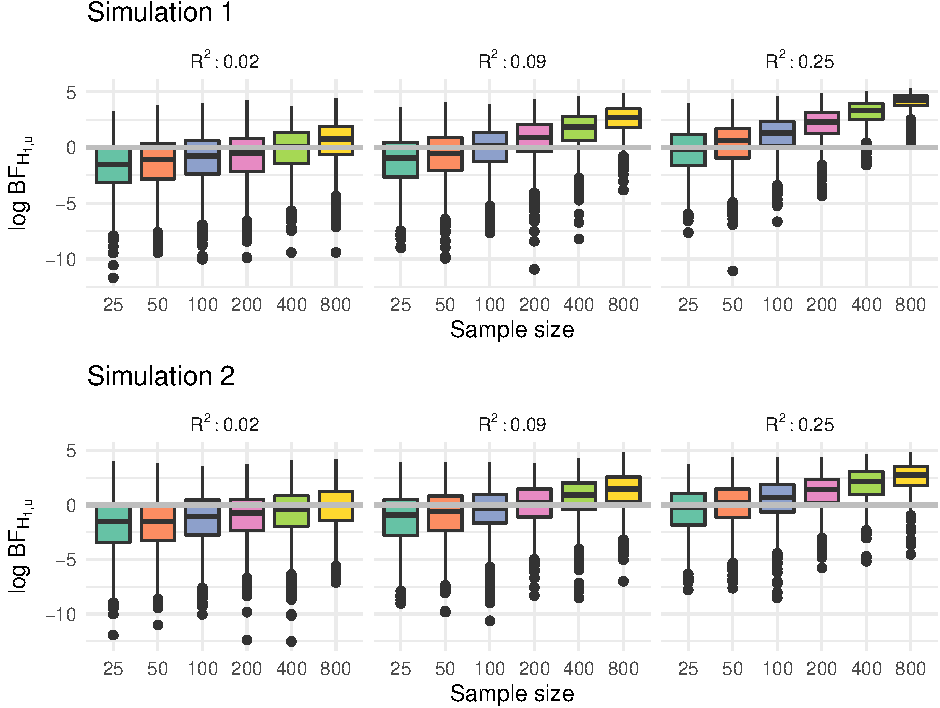
\includegraphics[width=1\linewidth]{research_report_volker_files/figure-latex/fig1-1} \caption{\label{fig1}Logarithm of the product of Bayes factors for the true hypothesis of interest versus an unconstrained hypothesis over three studies (generated with ordinary least squares (OLS), logistic and probit regression), for multiple sample sizes and effect sizes. In Simulation 2 the sample size of one randomly selected study is kept fixed at $n = 25$.}\label{fig:fig1}
\end{figure}

\begin{figure}
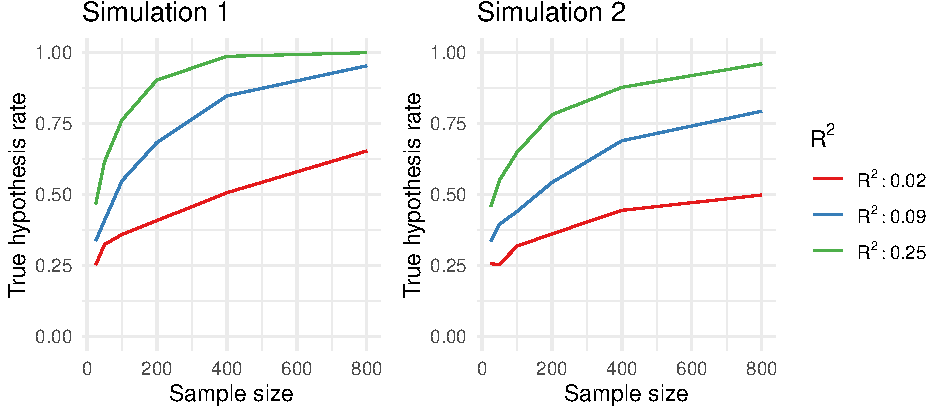
\includegraphics[width=1\linewidth]{research_report_volker_files/figure-latex/unnamed-chunk-2-1} \caption{\label{fig2}True hypothesis rate of $BES$ over three studies (generated with ordinary least squares (OLS), logistic and probit regression), for multiple sample sizes and effect sizes. In Simulation 2 the sample size of randomly selected study is kept fixed at $n = 25$.}\label{fig:unnamed-chunk-2}
\end{figure}

The simulations show that the aggregated Bayes factors generally tend to
increase with the sample size and effect size. In Simulation 1 in Figure
\ref{fig1}, the log-transformed product of Bayes factor over the three
studies \(\text{log}(BF_{1,u})\) is centered above zero only when the
sample size equals \(n = 800\) when the effect is small (i.e.,
\(R^2 = 0.02\)). Hence, with a small effect size, only the largest
sample size considered renders more support for \(\mathcal{H}_1\) than
for \(\mathcal{H}_u\) in the majority of the simulations. When
\(R^2 = 0.09\) or \(R^2 = 0.25\), \(\text{log}(BF_{1,u})\) is centered
around zero when \(n = 100\) and \(n = 25\), respectively, and shows
convincing support for the true hypothesis \(\mathcal{H}_1\) in nearly
all simulations for large sample sizes.

In Simulation 2 in Figure \ref{fig1}, where one of the three studies is
randomly selected to have a sample size of only \(n = 25\) observations,
\(\text{log}(BF_{1,u})\) is somewhat lower overall as compared to
Simulation 1 (ignoring those simulations in which the sample size of all
studies equals \(n = 25\)). This is to be expected, because with
\(n = 25\) the unconstrained hypothesis generally obtains more support
than hypothesis \(\mathcal{H}_1\), for all effect sizes. Apart from
this, a similar trend can be observed, in the sense that the aggregated
Bayes factors tend to increase with sample size and effect size.
However, the point from which the true hypothesis \(\mathcal{H}_1\)
receives most support in the majority of the simulations (i.e., the
point from which \(\text{log}(BF_{1,u})\) is centered above zero) is
generally reached later than in Simulation 1, and \(\mathcal{H}_1\) is
convincingly supported in most simulations only for large sample sizes
(i.e., \(n \geq 400\)) and a large effect (i.e., \(R^2 = 0.25\)).

A similar picture is shown in Figure \ref{fig2}, which displays the true
hypothesis rates for the hypothesis of interest \(\mathcal{H}_1\) using
the product of Bayes factors for both simulation set-ups. The true
hypothesis rate increases with the sample size and effect size. In
Simulation 1, when \(n = 25\) the true hypothesis receives most support
in only a minority of the simulations for all effect sizes, while for
\(n = 100\) only the studies with medium or large effects render most
support for \(\mathcal{H}_1\) in the majority of the simulations (i.e.,
about 50\% and 80\%, respectively). For \(n = 800\) all effect sizes
yield most support for the true hypothesis in the majority of
simulations. When the set of studies contains a single study with a
small sample size (i.e., \(n = 25\); in Simulation 2), the increase in
the true hypothesis rate is less steep and \(\mathcal{H}_1\) is
supported less often. Apart from this, the same general patterns can be
observed as in Simulation 1.

\hypertarget{discussion-and-conclusion}{%
\section{Discussion and conclusion}\label{discussion-and-conclusion}}

Overall, \emph{BES} showed to have satisfactory properties, in the sense
that it tends to select the true hypothesis when the power of the
studies is sufficiently large. In that sense, it proves to be a welcome
addition to conventional methods of research synthesis, like Bayesian
updating of parameter estimates or (Bayesian) meta-analysis. In contrast
to these methods, \emph{BES} can be applied when the study designs
differ (e.g., through the use of different statistical models, as
presented here). However, rather than pooled parameter estimates,
\emph{BES} provides the relative support for the hypotheses under
consideration over the entire set of studies simultaneously. That is,
\emph{BES} quantifies to what extent the theory of interest is supported
in each of these studies.

Consequently, unlike meta-analysis and Bayesian sequential updating,
which assess to what extent all studies together provide evidence for a
hypothesis, \emph{BES} cannot solve power issues. In fact, if the set of
studies contains a single, severely underpowered, study, this might
already affect the performance of \emph{BES}. Our second simulation
indeed suggests that including a single underpowered study, which is the
case for studies with a sample size of \(n = 25\) and a regression model
containing \(4\) predictors, lowers the performance of \emph{BES}
substantially. This finding warrants further research into the severity
of the effect of statistical power on the performance of \emph{BES}.
Moreover, it provides a cautionary note for researchers who want to
apply \emph{BES}: a synthesis of studies that lack statistical power
might yield invalid conclusions.

The current study focused exclusively on the effects of the sample size
and effect size on the performance of \emph{BES}. However, other factors
may likewise affect the outcome of \emph{BES}. When aggregating results
of different studies, the complexities of the study-specific hypotheses
may differ due different operationalizations of key variables. As Bayes
factors reflect a trade-off between the fit of the data to the
hypothesis and the complexity of the hypothesis, differences in
complexity may affect the outcome of \emph{BES}. Additionally, in our
simulations, we compared our hypothesis of interest with an
unconstrained alternative hypothesis. However, evaluating against the
classical null hypothesis, another informative hypothesis or the
complement hypothesis can be reasonable choices, too. To what extent
such factors will influence the performance of \emph{BES} is not yet
understood.

\bibliographystyle{tfcad}
\bibliography{../../thesis.bib}




\end{document}
